\documentclass{article}
\usepackage[utf8]{inputenc}
\usepackage[polish]{babel}
\usepackage{polski}
\usepackage{enumerate}
\usepackage{natbib}
\usepackage{graphicx}
\usepackage{geometry}
\newgeometry{tmargin=2.5cm, bmargin=2.5cm, lmargin=2.5cm, rmargin=2.5cm}
%wersja wyslana na eportal
\makeatletter
\newcommand{\linia}{\rule{\linewidth}{0.4mm}}
\renewcommand{\maketitle}{\begin{titlepage}
    \vspace*{1cm}
    \begin{center}
    Politechnika Wrocławska\\
    AiR ARR\\
 Projekt zespołowy
    \end{center}
      \vspace{3cm}
    \begin{center}

     \LARGE \textsc {\@title}
         \end{center}
     \vspace{1cm}

    \begin{center}
    \textit{ Autorzy:}\\
   \textit{\@author}
     \end{center}
      \vspace{1cm}

     \begin{center}

    Prowadzący:
  dr inż. Krzysztof Arent %dorobić inż mgr itd
    \end{center}

    \vspace*{\stretch{6}}
    \begin{center}
    \@date
    \end{center}
  \end{titlepage}
}
\makeatother
\author{Beata Berajter\\
Dawid Brząkała\\
Dorota Gidel\\
Katarzyna Wądrzyk\\
Ada Weiss\\
Małgorzata Witka-Jeżewska\\
 }%wpisać indeks
\title{SensGlove}

\begin{document}

\maketitle
\newpage
\tableofcontents
\newpage
\section{Opis projektu}
\subsection{Wstęp}
Celem projektu jest zbudowanie stanowiska do zbierania Bazy Danych biosygnałów oraz sygnałów z rękawiczki sensorycznej wchodzącej w interakcję z przedmiotami. Podjęcie tej tematyki umożliwi dalsze prace nad protezami kończyn górnych, w szczególności dłoni. Wyniki projektu wspomogą prace prowadzone nad protezami rąk, które ułatwiają wykonywanie codziennych czynności osobom niepełnosprawnym. Ważnym jest, aby proteza przy poruszaniu się przypominała prawdziwą kończynę w jak największym stopniu. Osiągnąć to można poprzez tworzenie bazy danych gdzie umieszczane będą interakcje palców ręki z różnymi przedmiotami codziennego użytku.
Badania te mogą zostać użyte nie tylko przy nowoczesnych protezach, lecz również przy budowie nowych, sprawniejszych robotów humanoidalnych.\\
Pierwszym krokiem przy realizacji projektu jest zapoznanie się z istniejącym już stanowiskiem do pomiarów, które umiejscowione jest na Politechnice Wrocławskiej, budynek C-3, sala 06. Po dogłębnym zaznajomieniu się z istniejącym już oprogramowaniem wykonamy nasze własne stanowisko badawcze, które składać się będzie z rękawiczki sensorycznej podłączonej poprzez mikrokontroler do karty, do której trafiają równocześnie pobierane biosygnały.\\
Efektem końcowym będzie stanowisko do poszerzania bazy danych zawierającej biosygnały oraz sygnały charakteryzujące interakcje palców protezy z przedmiotem.\\
Wyniki projektu będą upowszechniane przy pomocy strony internetowej (http://sensglove.happyrobotics.com/).\\


\subsection{Założenia projektowe}
W skład projektu wchodzą elementy takie jak:
\begin{itemize}
\item budowa rękawiczki z sensorami nacisku oraz ugięć
\item budowa interfejsu sprzętowego do obsługi sensorów rękawiczki - dostarczającego sygnały do karty pomiarowej
\item oprogramowanie do akwizycji danych
\item organizacja pomiarów prowadzących do utworzenia Bazy Danych
\item program do przedstawienia danych z czujników na ekranie graficznym
\end{itemize}
\subsection{Rozeznanie w dotychczasowych pracach}
\begin{itemize}
\item Maciej Przydatek, \textit{Wybrane metody przetwarzania biosygnałów}
\item Damian Brański,  \textit{Rejestracja i przetwarzanie sygnałów EMG i MMG}
\item Adam Krakowski, \textit{System sensoryczny dla cybernetycznej dłoni}
\end{itemize}

Prace te odnoszą się do istniejących w laboratorium 06 C3 projektów, jednym z nich jest projekt badania biosygnałów, który podobnie do projektu który chcemy zrealizować bada sygnały z czujników. System ten został stworzony do badania sygnałów w przedramieniu. Projekt pragniemy zrealizować tak, aby możliwe było w przyszłoci połączenie tych dwóch systemów i uzależnienie sygnałów w przedramieniu od odczytów sensorów nacisku i zgięcia w dłoni.

\section{Plan pracy}
\subsection{Poszczególne zdania}

\begin{enumerate}
    \item Zarządzanie projektem.
    \item Określenie wymagań użytkownika i kryteriów ewaluacji.
    \item Specyfikacja funkcjonalności,.
    \item Dekompozycja problemu na komponenty, architektura i kryteria ewaluacji komponentów. %Analiza wykonalnosci na nowej karcie, czas na zakup 2msc itd.
    \item Projekt i wykonanie bazy sprzętowo-programowej.
    \item Projekt komponentów:
    \begin{enumerate}[a)]
        \item wybór sensorów i projekt ich rozmieszczenia
        \item projekt interfejsu sprzętowego (schemat płytki + oprogramowanie układu z mikrokontrolerem)
        \item projekt oprogramowania akwizycji danych
        \item projekt bazy danych
        \item projekt programu do wizualizacji danych z czujników oraz biosygnałów

    \end{enumerate}
        \item Implementacja komponentów:
    \begin{enumerate}[a)]
        \item montaż sensorów na rękawiczce
        \item wykonanie płytki z mikrokontrolerem, montaż elementów elektronicznych, interfejs sprzętowy i uruchomienie, wytworzenie oprogramowania do obsługi mikrokontrolera
        \item wytworzenie oprogramowania do akwizycji danych
        \item wytworzenie zestawu zapytań do bazy danych
        \item wytworzenie programu do wizualizacji danych z czujników oraz biosygnałów


    \end{enumerate}
            \item Ewaluacja komponentów a-e:
    \item Integracja.
    \item Ewaluacja systemu.
    \item Upowszechnianie.
\end{enumerate}

\begin{figure}[h!]
\centering
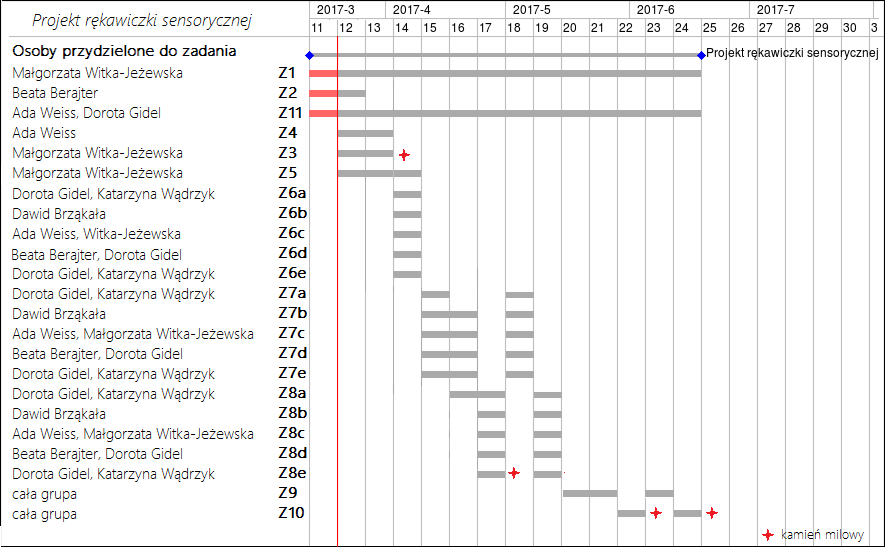
\includegraphics[scale=0.8]{projekt-rekawiczki-sensorycznej-gantt.png}
\caption{Diagram Gantt'a wraz z przypisaniem zadań do członków grupy}
\label{fig:projekt-rekawiczki-sensorycznej-gantt}
\end{figure}
\subsection{Kamienie milowe}
\begin{itemize}
\item 28.03 - oddanie raportu pierwszego
\item 02.05 - oddanie raportu drugiego
\item 16.05 - oddanie raportu trzeciego
\item 20.06 - oddanie ostatecznego raportu
\end{itemize}


\section{Doręczenie}
\begin{itemize}
\item raport pierwszy -  zawiera opisu projektu, specyfikację problemu, wyznaczone zadania i podział pracy - raport prywatny
\item raport drugi - zawiera dokumentację połączenia sensorów do płytki, kod źródłowy oprogramowania odbierającego i analizującego sygnały, kod źródłowy wizualizacji - raport prywatny
\item raport trzeci - zawiera raport z pierwszej ewaluacji zintegrowanego systemu - raport prywatny
\item raport ostateczny - zawiera dokumentację całościową projektu - raport publiczny
\end{itemize}


\section{Budżet}
\begin{center}
\begin{tabular}{|c|l|c|c|c|} \hline
    numer & nazwa & ilość & cena jednostkowa [zł] & cena całościowa [zł] \\ \hline
    1 & czujnik ugięcia & 6 & 30 & 180 \\
    2 & dotykowy czujnik nacisku & 1 & 80 & 80 \\
    3 & rękawiczka & 1 & 20 & 20 \\
    4 & przewody & 2 & 5 & 10 \\
    5 & elementy płytki & 1 & 60 & 60\\
    6 & opłata pracowników & 6 [os] & 27.15 /h & 34 209 *\\
    7 & wynajęcie pomieszczenia & 1 & 350/miesiąc & 1050 ** \\\hline
    \hline
    & & & Suma[zł] & 35 609\\
    \hline
\end{tabular}\\
\vspace{3mm}
\end{center}
* cana za wszystkich pracowników przez cały okres trwania projektu, zakładając pracę 15 godzin tygodniowo (3 godziny dziennie)\\
** cena wynajmu pomieszczenia za 3 miesiące


\section{Zarządzanie}
Rolę koordynatora projektu przyjęła Małgorzata Witka-Jeżewska. Każdy z członków zespołu otrzymuje zadanie, za które jest głównie odpowiedzialny oraz zadanie poboczne, w którym ma wspomóc osobę głównie odpowiedzialną za to zadanie. Koordynacja działań poszczególnych partnerów przeprowadzana jest poprzez program Redmine (prs-pwr.mooo.com). Ponadto w piątki od 9:15 do 13:00 organizowane będą spotkania mające na celu podsumowanie wyników pracy poszczególnych osób. Repozytorium grupy projektowej znajduje się na platformie GitHub.
\subsection{Zasady korzystania ze wspólnych zasobów}
Każdy członek zespołu ma równe prawa dostępu do plików zamieszczanych w repozytorium. Dodatkowo każdy z członków zespołu ma prawo korzystać ze stanowiska pomiarowego biosygnałów.
\subsection{Rozwiązywanie konfliktów}
Każda decyzja podejmowana jest poprzez głosowanie. Aby podjąć decyzję przynajmniej 4 osoby muszą opowiedzieć się za proponowanym rozwiązaniem. W przypadku podziału 3 za i 3 przeciw, głos koordynatora liczony jest podwójnie. Nie ma możliwości wstrzymania się od głosowania.
\subsection{Reguły przyznawania praw własności intelektualnej}
Projekt stanowi własność intelektualną każdego z członków grupy. Wszelkie decyzje podejmowane będą wg zasad opisanych w punkcie Rozwiązywanie konfliktów.
\section{Zespół}
\begin{itemize}
\item koordynator projektu: Małgorzata Witka-Jeżewska\\e-mail: 218634@student.pwr.wroc.pl\\
Zadania: zarządzanie projektem, specyfikacja funkcjonalności, oprogramowanie.
\item Beata Berajter \\
Zadania: określenie wymagań użytkownika, bazy danych.
\item Dawid Brząkała \\
Zadania: interfejs.
\item Dorota Gidel \\
Zadania: rękawiczka, wizualizacja, upowszechnianie, bazy danych.
\item Katarzyna Wądrzyk \\
Zadania: rękawiczka i sensory, wizualizacja.
\item Ada Weiss \\
Zadania: dekompozycja, oprogramowanie, upowszechnianie.
\end{itemize}
\end{document}
